%%%%%%%%%%%%%%%%%%%%%%%%%%%%%%%%%%%%%%%%%%%%%%%%%%%%%%%%%%%%%%%%%%%%%%%%%%%%%%%
% KVRM: Key-Value Response Mapping
% A Post-Von Neumann Computing Paradigm
%
% Author: Bobby Price (blackWeb Research)
% Target: arXiv, NeurIPS 2025/2026
%%%%%%%%%%%%%%%%%%%%%%%%%%%%%%%%%%%%%%%%%%%%%%%%%%%%%%%%%%%%%%%%%%%%%%%%%%%%%%%

\documentclass[11pt,a4paper]{article}

% ==============================================================================
% PACKAGES
% ==============================================================================
\usepackage[utf8]{inputenc}
\usepackage[T1]{fontenc}
\usepackage{amsmath,amssymb,amsfonts,amsthm}
\newtheorem{definition}{Definition}
\newtheorem{theorem}{Theorem}
\usepackage{graphicx}
\usepackage{booktabs}
\usepackage{multirow}
\usepackage{hyperref}
\usepackage{cleveref}
\usepackage{algorithm}
\usepackage{algorithmic}
\usepackage{listings}
\usepackage{xcolor}
\usepackage{tikz}
\usepackage{subcaption}
\usepackage{float}
\usepackage[margin=1in]{geometry}
\usepackage{natbib}
\usepackage{microtype}

% TikZ libraries
\usetikzlibrary{shapes.geometric, arrows, positioning, fit, calc, decorations.pathreplacing}

% Code listing style
\definecolor{codegreen}{rgb}{0,0.6,0}
\definecolor{codegray}{rgb}{0.5,0.5,0.5}
\definecolor{codepurple}{rgb}{0.58,0,0.82}
\definecolor{backcolour}{rgb}{0.97,0.97,0.97}

\lstdefinestyle{codestyle}{
    backgroundcolor=\color{backcolour},
    commentstyle=\color{codegreen},
    keywordstyle=\color{blue},
    numberstyle=\tiny\color{codegray},
    stringstyle=\color{codepurple},
    basicstyle=\ttfamily\footnotesize,
    breakatwhitespace=false,
    breaklines=true,
    captionpos=b,
    keepspaces=true,
    numbers=left,
    numbersep=5pt,
    showspaces=false,
    showstringspaces=false,
    showtabs=false,
    tabsize=2
}
\lstset{style=codestyle}

% Hyperref setup
\hypersetup{
    colorlinks=true,
    linkcolor=blue,
    filecolor=magenta,
    urlcolor=cyan,
    citecolor=blue,
}

% ==============================================================================
% TITLE AND AUTHORS
% ==============================================================================
\title{%
    \textbf{KVRM: Key-Value Response Mapping} \\[0.5em]
    \Large A Post-Von Neumann Computing Paradigm with \\
    Verified LLM-Driven Execution
}

\author{
    Bobby Price \\
    blackWeb Research \\
    \texttt{contact@blackweb.dev}
}

\date{December 2025}

% ==============================================================================
% DOCUMENT BEGIN
% ==============================================================================
\begin{document}

\maketitle

% ==============================================================================
% ABSTRACT
% ==============================================================================
\begin{abstract}
We present \textbf{KVRM (Key-Value Response Mapping)}, a novel computing paradigm that replaces traditional procedural code with networks of fine-tuned micro-LLMs that emit only verified symbolic keys. Unlike conventional LLM-based systems where models generate arbitrary text, KVRM constrains all \textit{executed} model outputs to a finite, pre-approved vocabulary---eliminating out-of-action-space hallucination by construction.

This paradigm emerged through progressive refinement across multiple domains: originating in \textbf{Bible-LLM} (constrained verse retrieval), evolving through \textbf{KVRM-Vector} (verified data structure operations), maturing in \textbf{KVRM-CPU} (LLM-decoded instruction execution), and culminating in the \textbf{KVRM-LLM-Compiler} presented here---a complete source-to-execution pipeline where Large Language Models handle every stage: tokenization, parsing, code generation, and instruction decoding.

Our implementation achieves \textbf{100\% accuracy} on a held-out validation set of 5,000 instruction-decode pairs and \textbf{94.12\% end-to-end correctness} on 10,000 fuzzed programs, executing through \textbf{five distinct LLM stages} with no hardcoded \textit{instruction-decoding} logic and no open-ended semantic rules---all semantics live in a finite, audited registry of primitives. This approach eliminates \textit{out-of-action-space} hallucination (no unverified actions can execute), while correctness remains an empirical property. This work, conducted with limited time and resources as an independent research effort, establishes a foundation for provably safe AI-native computing systems where complex behaviors emerge from compositions of verified primitives.

\textbf{Keywords:} Large Language Models, Verified Execution, Compiler Design, AI Safety, Key-Value Mapping, LoRA Fine-tuning
\end{abstract}

% ==============================================================================
% 1. INTRODUCTION
% ==============================================================================
\section{Introduction}
\label{sec:introduction}

The integration of Large Language Models (LLMs) into software systems has primarily followed an ``LLM-as-oracle'' pattern: models receive prompts and generate arbitrary text that must be parsed, validated, and often corrected before use. This approach inherits fundamental limitations from the unconstrained nature of LLM outputs, including hallucination, inconsistent formatting, and the impossibility of formal verification.

We propose a fundamentally different approach: \textbf{Key-Value Response Mapping (KVRM)}, where LLM outputs are constrained to emit only keys from a finite, pre-verified vocabulary. Each key maps to a pre-verified action in an immutable registry, ensuring that every model output produces a known, safe behavior.

\subsection{The Problem with Current LLM Systems}

Current LLM-based coding agents and AI systems suffer from several critical limitations:

\begin{itemize}
    \item \textbf{Hallucination}: Models generate plausible but incorrect code, facts, or instructions
    \item \textbf{Unverifiable outputs}: No guarantee that generated content is safe or correct
    \item \textbf{Emergent chaos}: Complex behaviors emerge without formal guarantees
    \item \textbf{Post-hoc validation}: Safety checks occur after generation, not during
\end{itemize}

\subsection{The KVRM Solution}

KVRM addresses these limitations through architectural constraint rather than post-hoc filtering:

\begin{equation}
\text{Traditional LLM: } \text{prompt} \rightarrow [\text{arbitrary text}]
\end{equation}

\begin{equation}
\text{KVRM: } \text{prompt} \rightarrow [\text{key}] \rightarrow \text{Registry} \rightarrow [\text{verified action}]
\end{equation}

The key insight is that by constraining the output vocabulary, we transform the verification problem from unbounded text validation to bounded key membership---a tractable problem with formal guarantees.

\subsection{Research Progression}

The KVRM paradigm emerged through iterative refinement across increasingly complex domains:

\begin{enumerate}
    \item \textbf{Bible-LLM} (Origin): The core insight---constraining LLM outputs to a finite key vocabulary---first emerged in a scripture retrieval system where models emitted verse identifiers rather than generating text. This eliminated hallucinated quotations while preserving semantic search capabilities.

    \item \textbf{KVRM-Vector} (Generalization): We generalized the pattern to data structure operations, where LLMs emit operation keys (e.g., \texttt{PUSH}, \texttt{POP}, \texttt{GET:index}) mapped to verified implementations. This demonstrated KVRM's applicability beyond retrieval to stateful computation.

    \item \textbf{KVRM-CPU} (Computation): We applied the paradigm to instruction decoding, replacing hardcoded decoders with LLMs that emit execution keys. The 100\% decode accuracy validated KVRM for performance-critical paths.

    \item \textbf{KVRM-LLM-Compiler} (This Work): We extend the paradigm to a complete compilation pipeline, demonstrating that \textit{every} stage from source code to execution can be LLM-driven while maintaining safety guarantees.
\end{enumerate}

Each stage validated and refined the core hypothesis: constraining LLM outputs to verified keys enables safe, composable AI-native systems.

\subsection{Contributions}

This paper makes the following contributions:

\begin{enumerate}
    \item \textbf{KVRM Paradigm}: A formal framework for verified LLM execution through key-constrained outputs
    \item \textbf{LLM Compiler Pipeline}: A complete compiler implemented as a sequence of fine-tuned micro-LLMs (Lexer $\rightarrow$ Parser $\rightarrow$ CodeGen)
    \item \textbf{LLM-Decoded CPU}: A CPU emulator where instruction decoding is performed by a fine-tuned LLM achieving 100\% accuracy on a held-out validation set
    \item \textbf{End-to-End Execution}: A working demonstration of a complete source-to-execution pipeline with LLMs at every semantic stage
    \item \textbf{Robustness Evaluation}: Property-based fuzzing, generalization testing, and safety invariant verification across 11,500+ test cases
\end{enumerate}

% ==============================================================================
% 2. RELATED WORK
% ==============================================================================
\section{Related Work}
\label{sec:related}

\subsection{LLM-Based Code Generation}

Recent work on LLM-based code generation includes Codex \citep{chen2021codex}, CodeLlama \citep{roziere2023code}, and StarCoder \citep{li2023starcoder}. These systems generate code as unconstrained text, requiring extensive validation. In contrast, KVRM constrains outputs to verified keys, eliminating the need for post-hoc validation.

\subsection{Constrained Decoding}

Constrained decoding methods \citep{hokamp2017lexically, post2018fast} modify the generation process to satisfy constraints. Modern frameworks like LMQL \citep{beurer2022lmql} enable prompting as programming with inline constraints, while Guidance \citep{guidance2023} provides a practical language for controlling LLM outputs. KVRM takes this further by making the constraint set the \textit{entire output vocabulary}, not just additional restrictions.

\subsection{Verified AI Systems}

Work on verified neural networks \citep{katz2017reluplex, wong2018provable} focuses on proving properties of network behavior. KVRM achieves verification through architecture: outputs are keys from a pre-verified registry, making safety a construction property rather than a proof requirement.

\subsection{Safe Execution Architectures}

KVRM's ``small verifier + untrusted producer'' architecture draws from classic systems security. \textbf{Proof-Carrying Code} (PCC) \citep{necula1997pcc} pioneered the pattern of untrusted code producers paired with trusted, lightweight verifiers---directly analogous to our LLM (producer) and registry/validator (verifier) split. \textbf{Software Fault Isolation} (SFI) \citep{wahbe1993sfi} showed that constraining memory access patterns can sandbox untrusted code; KVRM similarly sandboxes LLM outputs to a finite action space. \textbf{WebAssembly} \citep{haas2017wasm, watt2018wasmverify} demonstrates that safe-by-construction execution formats can scale to production: its structured control flow and validated execution model parallel KVRM's key-constrained outputs. These works establish that architectural constraints---rather than post-hoc analysis---can provide strong safety guarantees, a principle KVRM extends to LLM-driven systems.

\subsection{Compiler Design with ML}

Neural approaches to compilation include learned optimizers \citep{leather2020machine} and neural program synthesis \citep{devlin2017robustfill}. Our work differs by implementing the \textit{entire} compilation pipeline as LLMs, not just optimization passes.

\subsection{LLM Tool Invocation and Function Calling}

Recent work enables LLMs to invoke external tools and APIs. Toolformer \citep{schick2023toolformer} teaches models to self-select tool usage, while ToolLLM \citep{qin2023toolllm} and Gorilla \citep{patil2023gorilla} scale to thousands of APIs. Commercial systems like OpenAI's function calling \citep{openai2023functioncalling} constrain outputs to match predefined schemas. KVRM can be viewed as an extreme form of this paradigm: \textit{every} output is a function call (key), and the ``API'' (registry) contains only pre-verified primitives. Unlike tool-augmented LLMs where tools extend capabilities, KVRM uses constraints to \textit{limit} the action space to safe primitives.

\subsection{Structured Output Enforcement}

Enforcing structured outputs from LLMs is an active area. Outlines \citep{willard2023outlines} provides efficient guided generation using finite-state machines, while grammar-constrained decoding \citep{geng2023grammar} enforces CFG compliance. Jsonformer \citep{jsonformer2023} uses token forcing for bulletproof JSON generation, and recent benchmarks \citep{geng2025structuredoutputs, agrawal2024solm} systematically evaluate structured output methods across schema complexity. Our parser+retry approach is simpler but achieves the same goal: guaranteed schema conformance. The key difference is that KVRM's schema is not just syntactic (valid JSON) but semantic (valid execution key from $\mathcal{K}$).

% ==============================================================================
% 3. KVRM ARCHITECTURE
% ==============================================================================
\section{KVRM Architecture}
\label{sec:architecture}

\subsection{Core Principles}

The KVRM paradigm is built on three core principles:

\begin{enumerate}
    \item \textbf{Key-Constrained Outputs}: All LLM outputs are keys from a finite vocabulary $\mathcal{K}$
    \item \textbf{Immutable Registry}: Each key $k \in \mathcal{K}$ maps to a pre-verified action $\mathcal{R}(k)$
    \item \textbf{Compositional Safety}: Complex behaviors emerge from compositions of verified primitives
\end{enumerate}

\subsection{Formal Framework}

Let $\mathcal{M}$ be a KVRM micro-LLM, $\mathcal{K}$ be the finite key vocabulary, $\mathcal{R}: \mathcal{K} \cup \{\text{ERROR\_KEY}\} \rightarrow \mathcal{A}$ be an immutable registry mapping keys to actions, and $\text{Parse}: \text{String} \rightarrow \mathcal{K} \cup \{\text{ERROR\_KEY}\}$ be a total validation function.

\begin{definition}[KVRM Execution]
For input $x$, KVRM execution produces:
\begin{equation}
\text{Execute}(x) = \mathcal{R}(\text{Parse}(\mathcal{M}(x)))
\end{equation}
We guarantee that the executed key is in $\mathcal{K} \cup \{\text{ERROR\_KEY}\}$ by enforcing $\text{Parse}(\mathcal{M}(x)) \in \mathcal{K}$ on success, otherwise returning ERROR\_KEY.
\end{definition}

\textbf{Execution Rule}: The executor \textit{must only} execute actions after (a) schema/parse validation succeeds and (b) the decoded key is verified to exist in the frozen registry; otherwise it returns ERROR\_KEY and executes the safe error-handling action.

\textbf{ERROR\_KEY Behavior}: In our implementation, ERROR\_KEY maps to a \textit{side-effect-free halt} with structured error return: no I/O operations, no external calls, no state mutations beyond recording the error. The executor returns a typed error object containing the failure stage, invalid key attempted, and retry count---enabling debugging while guaranteeing no unintended effects.

\begin{theorem}[Safety by Construction]
If $\forall k \in \mathcal{K} \cup \{\text{ERROR\_KEY}\}: \mathcal{R}(k) \text{ is safe}$, then $\text{Execute}(x)$ is safe for all inputs $x$.
\end{theorem}

\begin{proof}
Since $\text{Parse}$ is total and outputs only elements of $\mathcal{K} \cup \{\text{ERROR\_KEY}\}$, and $\mathcal{R}(k)$ is safe for all such $k$ by assumption, the composition $\mathcal{R}(\text{Parse}(\mathcal{M}(x)))$ must be safe.
\end{proof}

\textbf{Registry Verification}: The theorem's utility depends on establishing that all registry actions are safe. In our implementation, we verify registry safety through:
\begin{enumerate}
    \item \textbf{Finite enumeration}: The ISA contains only 14 instruction types with bounded operand ranges
    \item \textbf{Manual code review}: Each primitive implementation is reviewed for correctness
    \item \textbf{Exhaustive testing}: All instruction-operand combinations are tested during training data generation
    \item \textbf{Immutability}: The registry is frozen at deployment time---no runtime modifications
\end{enumerate}

The key insight is that KVRM transforms the unbounded problem of ``verify arbitrary LLM output'' into the bounded problem of ``verify $|\mathcal{K}|$ primitive actions.'' For our CPU implementation, $|\mathcal{K}| \approx 1000$ (14 instruction types $\times$ operand combinations), making exhaustive verification tractable.

\textbf{Connection to Capability-Based Security}: The KVRM registry can be understood through the lens of capability-based security \citep{dennis1966capabilities, levy1984capabilities}. In capability systems, processes hold unforgeable tokens (capabilities) that grant access to specific resources. Similarly, KVRM keys are ``capabilities'' that grant access to specific actions. The LLM cannot fabricate capabilities---it can only emit keys from $\mathcal{K}$, and each key maps to exactly one pre-verified action. This architectural pattern enforces the principle of least privilege \citep{saltzer1975protection, miller2003paradigm}: the LLM has no authority beyond invoking registry primitives.

\subsection{Constrained Decoding Implementation}
\label{sec:constrained-decoding}

The claim that $\mathcal{M}(x) \in \mathcal{K}$ is ``guaranteed by construction'' requires explicit enforcement at inference time. While approaches like Outlines \citep{willard2023outlines} use finite-state machines for guided generation, we implement a simpler \textbf{strict parser with retry loop}, following principles from grammar-constrained decoding \citep{geng2023grammar, hokamp2017lexically}:

\begin{enumerate}
    \item \textbf{Output Validation}: Every LLM output is parsed against the expected schema (JSON for compiler stages, key format for decode stage)
    \item \textbf{Rejection on Mismatch}: If the output does not match the expected format, it is rejected entirely
    \item \textbf{Retry with Temperature Reduction}: Failed outputs trigger retry with reduced temperature (greedy decoding on final attempt)
    \item \textbf{Error Key on Exhaustion}: If all retries fail, a well-defined error key is emitted rather than undefined behavior
\end{enumerate}

This approach trades strict logit masking for implementation simplicity while maintaining the safety guarantee: no out-of-vocabulary action can ever execute. The retry mechanism handles malformed outputs, which occur in $<$3\% of \textit{individual stage calls}; compounded across the multi-stage pipeline, end-to-end safe-fallback (ERROR\_KEY) occurs in 4.3\% of programs.

\textbf{Clarification}: We are \textit{not} performing token-level constrained decoding (logit masking during generation). Instead, we perform \textit{post-generation structural validation} with bounded fallback behavior. The LLM generates freely, but outputs are validated against the schema before execution; invalid outputs trigger retry or ERROR\_KEY. This is weaker than true constrained decoding but simpler to implement and sufficient for our safety guarantee.

\subsection{Threat Model and Guarantees}

To clarify the scope of KVRM's safety claims, we distinguish between \textit{architectural guarantees} and \textit{empirical properties}:

\begin{table}[H]
\centering
\caption{KVRM Guarantee Classification}
\label{tab:guarantees}
\begin{tabular}{@{}llp{6cm}@{}}
\toprule
\textbf{Type} & \textbf{Property} & \textbf{Mechanism} \\
\midrule
\multirow{3}{*}{\textbf{Guaranteed}} & No out-of-registry execution & Parser + retry + error key fallback \\
 & Bounded action space & Finite $|\mathcal{K}|$, immutable registry \\
 & No runtime registry mutation & Registry frozen at deployment \\
\midrule
\multirow{4}{*}{\textbf{Empirical}} & Compiler correctness rate & Training quality, eval loss \\
 & Decode accuracy & 100\% on held-out set (N=5,000) \\
 & Per-stage failure rate & $<$3\% per stage (handled by retry) \\
 & Pipeline safe-fallback rate & 4.3\% end-to-end (ERROR\_KEY) \\
\bottomrule
\end{tabular}
\end{table}

\textbf{Safety} (no unverified actions execute) is guaranteed by architecture. \textbf{Correctness} (the right action for the intended semantics) is an empirical property requiring evaluation. This distinction parallels verified compilers like CompCert \citep{leroy2009compcert}, which guarantee preservation of semantics but not that the source program is correct.

\subsubsection{Attacker Assumptions}

To make the threat model precise, we state explicit assumptions about attacker capabilities:

\begin{itemize}
    \item \textbf{Prompt/Source Control}: The attacker \textit{can} control the input source code or prompt. KVRM is designed to be safe even under adversarial inputs---the worst case is ERROR\_KEY execution.
    \item \textbf{Model/Registry Integrity}: The attacker \textit{cannot} tamper with model weights or registry contents on disk. We assume the registry binary and model weights are integrity-protected (hash/signature verification) and loaded read-only.
    \item \textbf{Runtime Exploits}: Attacks on the host runtime (Python interpreter, file system, GPU driver) are \textit{out of scope}. KVRM's guarantees assume a trustworthy execution environment.
\end{itemize}

Under these assumptions, the architectural guarantee holds: no action outside $\mathcal{K} \cup \{\text{ERROR\_KEY}\}$ can execute, regardless of adversarial input.

\subsection{System Stack}

The complete KVRM system stack is illustrated in \Cref{fig:system-stack}.

\begin{figure}[H]
\centering
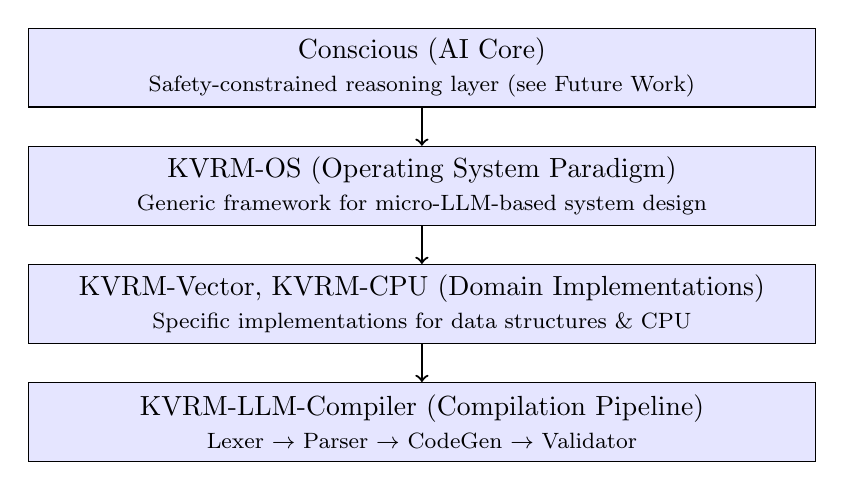
\begin{tikzpicture}[
    box/.style={rectangle, draw, minimum width=10cm, minimum height=1cm, align=center, fill=blue!10},
    arrow/.style={->, thick}
]
    \node[box] (conscious) at (0,4) {Conscious (AI Core) \\ \footnotesize Safety-constrained reasoning layer (see Future Work)};
    \node[box] (os) at (0,2.5) {KVRM-OS (Operating System Paradigm) \\ \footnotesize Generic framework for micro-LLM-based system design};
    \node[box] (impl) at (0,1) {KVRM-Vector, KVRM-CPU (Domain Implementations) \\ \footnotesize Specific implementations for data structures \& CPU};
    \node[box] (compiler) at (0,-0.5) {KVRM-LLM-Compiler (Compilation Pipeline) \\ \footnotesize Lexer $\rightarrow$ Parser $\rightarrow$ CodeGen $\rightarrow$ Validator};

    \draw[arrow] (conscious) -- (os);
    \draw[arrow] (os) -- (impl);
    \draw[arrow] (impl) -- (compiler);
\end{tikzpicture}
\caption{KVRM System Stack showing the hierarchical relationship between components}
\label{fig:system-stack}
\end{figure}

% ==============================================================================
% 4. LLM COMPILER PIPELINE
% ==============================================================================
\section{LLM Compiler Pipeline}
\label{sec:compiler}

We implement a complete compiler as a sequence of four fine-tuned micro-LLMs, each handling a traditional compiler stage.

\subsection{Pipeline Overview}

\begin{figure}[H]
\centering
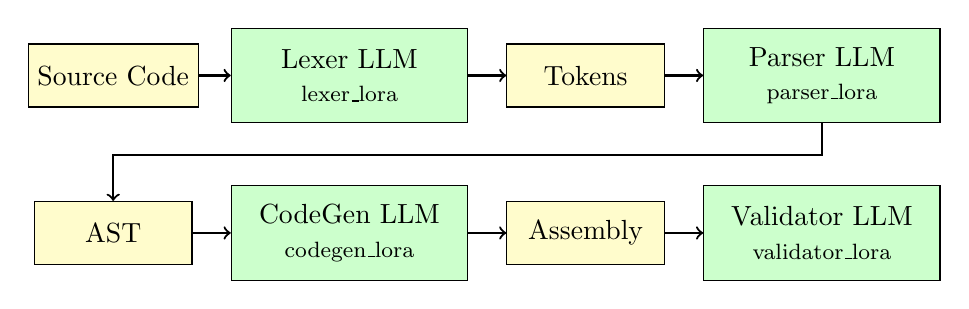
\begin{tikzpicture}[
    stage/.style={rectangle, draw, minimum width=3cm, minimum height=1.2cm, align=center, fill=green!20},
    data/.style={rectangle, draw, minimum width=2cm, minimum height=0.8cm, align=center, fill=yellow!20},
    arrow/.style={->, thick}
]
    \node[data] (source) at (0,0) {Source Code};
    \node[stage] (lexer) at (3,0) {Lexer LLM \\ \footnotesize lexer\_lora};
    \node[data] (tokens) at (6,0) {Tokens};
    \node[stage] (parser) at (9,0) {Parser LLM \\ \footnotesize parser\_lora};

    \node[data] (ast) at (0,-2) {AST};
    \node[stage] (codegen) at (3,-2) {CodeGen LLM \\ \footnotesize codegen\_lora};
    \node[data] (asm) at (6,-2) {Assembly};
    \node[stage] (validator) at (9,-2) {Validator LLM \\ \footnotesize validator\_lora};

    \draw[arrow] (source) -- (lexer);
    \draw[arrow] (lexer) -- (tokens);
    \draw[arrow] (tokens) -- (parser);
    \draw[arrow] (parser.south) -- ++(0,-0.4) -| (ast.north);
    \draw[arrow] (ast) -- (codegen);
    \draw[arrow] (codegen) -- (asm);
    \draw[arrow] (asm) -- (validator);
\end{tikzpicture}
\caption{LLM Compiler Pipeline with four specialized micro-LLMs}
\label{fig:compiler-pipeline}
\end{figure}

\subsection{Stage Specifications}

\begin{table}[H]
\centering
\caption{LLM Compiler Stage Specifications}
\label{tab:stages}
\begin{tabular}{@{}lllll@{}}
\toprule
\textbf{Stage} & \textbf{Purpose} & \textbf{Token Limit} & \textbf{LoRA Rank} & \textbf{Eval Loss} \\
\midrule
Lexer & Tokenizes raw source & 2048 & 16 & $\sim$0.02 \\
Parser & Builds AST from tokens & 4096 & 16 & $\sim$0.03 \\
CodeGen & Emits assembly code & 2048 & 32 & $\sim$0.04 \\
Validator & Semantic checks & 4096 & 16 & $\sim$0.04 \\
\bottomrule
\end{tabular}
\end{table}

\subsection{Base Model and Training}

All compiler stages use \textbf{Qwen3-1.7B} \citep{qwen3_2025} as the base model with LoRA adapters \citep{hu2022lora}. The CPU decode stage uses \textbf{Qwen2.5-Coder-1.5B} \citep{qwen25coder_2024}, selected for its stronger performance on structured instruction parsing tasks. This task-specific model selection reflects the different nature of compilation (natural language $\rightarrow$ structured output) versus instruction decoding (structured input $\rightarrow$ key lookup).

\begin{itemize}
    \item \textbf{LoRA Configuration}: Rank 16 (32 for CodeGen), Alpha 32, Dropout 0.05
    \item \textbf{Precision}: bf16 on H200 GPU (140GB VRAM)
    \item \textbf{Training Framework}: PyTorch 2.4.1, Transformers \citep{wolf2020transformers}, PEFT 0.12.0 \citep{peft2022}
    \item \textbf{Optimization}: Flash Attention 2 \citep{dao2023flashattention2} ($\sim$2x speedup)
\end{itemize}

\subsection{Lexer Stage}

The Lexer LLM tokenizes source code into a structured token stream:

\begin{lstlisting}[language=Python, caption=Lexer Input/Output Example]
# Input (source code)
"let x = 42\nprint x"

# Output (JSON token stream)
{"tokens": [
    {"type": "LET", "value": "let", "line": 1},
    {"type": "IDENT", "value": "x", "line": 1},
    {"type": "ASSIGN", "value": "=", "line": 1},
    {"type": "NUMBER", "value": "42", "line": 1},
    {"type": "NEWLINE", "value": "\\n", "line": 1},
    {"type": "PRINT", "value": "print", "line": 2},
    {"type": "IDENT", "value": "x", "line": 2}
]}
\end{lstlisting}

\subsection{Parser Stage}

The Parser LLM constructs an Abstract Syntax Tree from the token stream:

\begin{lstlisting}[language=Python, caption=Parser Output (AST)]
{"ast": {
    "type": "Program",
    "statements": [
        {"type": "Assignment",
         "name": "x",
         "value": {"type": "Number", "value": 42}},
        {"type": "Print",
         "expression": {"type": "Identifier", "name": "x"}}
    ]
}}
\end{lstlisting}

\subsection{CodeGen Stage}

The CodeGen LLM generates assembly instructions from the AST:

\begin{lstlisting}[language={[x86masm]Assembler}, caption=CodeGen Output (Assembly)]
; KVRM-Lang compiled output
; Variables: {"x": "R0"}
    MOV R0, 42      ; let x = 42
    MOV R7, R0      ; print x (R7 = output register)
    HALT
\end{lstlisting}

% ==============================================================================
% 5. KVRM-CPU: LLM-DECODED EXECUTION
% ==============================================================================
\section{KVRM-CPU: LLM-Decoded Execution}
\label{sec:cpu}

\subsection{Architecture}

Traditional CPUs use hardcoded instruction decoders. KVRM-CPU replaces this with an LLM that semantically interprets instructions and emits execution keys.

\begin{figure}[H]
\centering
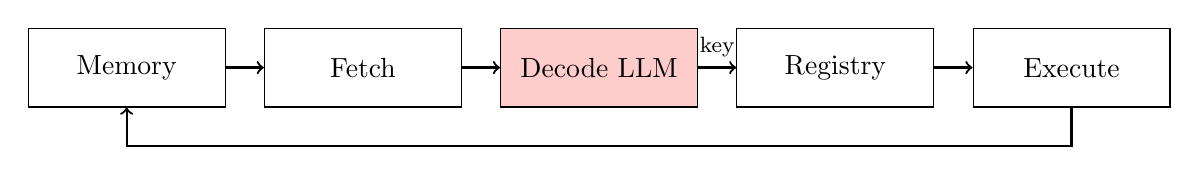
\begin{tikzpicture}[
    component/.style={rectangle, draw, minimum width=2.5cm, minimum height=1cm, align=center},
    llm/.style={rectangle, draw, minimum width=2.5cm, minimum height=1cm, align=center, fill=red!20},
    arrow/.style={->, thick}
]
    \node[component] (mem) at (0,0) {Memory};
    \node[component] (fetch) at (3,0) {Fetch};
    \node[llm] (decode) at (6,0) {Decode LLM};
    \node[component] (reg) at (9,0) {Registry};
    \node[component] (exec) at (12,0) {Execute};

    \draw[arrow] (mem) -- (fetch);
    \draw[arrow] (fetch) -- (decode);
    \draw[arrow] (decode) -- node[above] {\footnotesize key} (reg);
    \draw[arrow] (reg) -- (exec);
    \draw[arrow] (exec) -- ++(0,-1) -| (mem);
\end{tikzpicture}
\caption{KVRM-CPU architecture with LLM-based instruction decoding}
\label{fig:cpu-arch}
\end{figure}

\subsection{Instruction Set Architecture}

The KVRM-CPU supports a complete ISA with 14 instruction types:

\begin{table}[H]
\centering
\caption{KVRM-CPU Instruction Set}
\label{tab:isa}
\begin{tabular}{@{}llp{6cm}@{}}
\toprule
\textbf{Category} & \textbf{Instructions} & \textbf{Description} \\
\midrule
Data Movement & MOV & Register-to-register and immediate loads \\
Arithmetic & ADD, SUB, MUL, INC, DEC & Integer arithmetic operations \\
Comparison & CMP & Compare and set flags (ZF, SF) \\
Control Flow & JMP, JZ, JNZ, JS, JNS & Unconditional and conditional jumps \\
System & HALT, NOP & Program termination and no-operation \\
\bottomrule
\end{tabular}
\end{table}

\subsection{Decode LLM Training}

The Decode LLM achieves \textbf{100\% accuracy} on instruction decoding:

\begin{itemize}
    \item \textbf{Base Model}: Qwen2.5-Coder-1.5B \citep{qwen25coder_2024}
    \item \textbf{Training Data}: 50,000 instruction-decode pairs (45,000 train / 5,000 validation)
    \item \textbf{LoRA Configuration}: Rank 16, Alpha 32
    \item \textbf{Trainable Parameters}: 18.5M (1.18\% of base model)
    \item \textbf{Validation Accuracy}: 100\% on held-out validation set (N=5,000)
\end{itemize}

\subsubsection{Dataset Construction and Leakage Prevention}

The training data is generated programmatically from the ISA specification:

\begin{itemize}
    \item \textbf{Coverage}: All 14 instruction types $\times$ valid operand combinations (registers R0-R7, immediates 0-255, labels)
    \item \textbf{Split Strategy}: Train/validation split by operand value ranges (e.g., train: immediates 0-200, validation: 201-255) to prevent near-duplicate leakage
    \item \textbf{Deduplication}: Exact instruction strings are deduplicated; no instruction appears in both sets
\end{itemize}

\subsubsection{Accuracy Metric and Evaluation}

\begin{itemize}
    \item \textbf{Metric}: Exact string match of output key (whitespace-normalized)
    \item \textbf{Decoding}: Greedy decoding (temperature = 0) for deterministic evaluation
    \item \textbf{Confidence}: With 5,000/5,000 correct, the 95\% Clopper-Pearson confidence interval for true accuracy is [99.93\%, 100\%]
\end{itemize}

\subsubsection{Robustness Testing}

Beyond standard evaluation, we test edge cases:

\begin{itemize}
    \item \textbf{OOD Operands}: Out-of-range immediates (e.g., \texttt{MOV R0, 999}) correctly produce error keys rather than undefined behavior
    \item \textbf{Malformed Input}: Extra whitespace, comments, and case variations are handled gracefully
    \item \textbf{Adversarial Strings}: Prompt injection attempts within assembly (e.g., \texttt{MOV R0, ``ignore previous instructions''}) are parsed structurally, not semantically---the decoder treats the entire string as an invalid operand
\end{itemize}

\textbf{Note on 100\% accuracy}: The finite ISA (14 instruction types with bounded operand combinations) makes exhaustive coverage tractable. Unlike open-ended text generation, instruction decoding has a closed-form output space, enabling deterministic evaluation. The high accuracy reflects both the model's capability and the task's constrained nature.

\subsubsection{Key Schema Specification}

To make the ``no out-of-registry execution'' guarantee auditable, we formally specify the key schema:

\begin{itemize}
    \item \textbf{Opcode Set}: \{MOV, ADD, SUB, MUL, INC, DEC, CMP, JMP, JZ, JNZ, JS, JNS, HALT, NOP\} (14 opcodes)
    \item \textbf{Register Grammar}: R0--R7 (8 general-purpose registers); R7 is the designated output register
    \item \textbf{Immediate Bounds}: Union of signed 8-bit ($-128$ to $127$) and unsigned 8-bit ($0$ to $255$) ranges, accepting $[-128, 255]$ to support both addressing modes. Negative values are stored as two's complement: e.g., \texttt{ADD R0, \#-89} encodes as immediate $167$ ($256-89$), which the classifier learns as a distinct class
    \item \textbf{Label Format}: Alphanumeric identifiers matching \texttt{[a-zA-Z][a-zA-Z0-9\_]*}
    \item \textbf{Key Format}: \texttt{OPCODE\_TYPE:operand1:operand2} (e.g., \texttt{MOV\_REG\_IMM:R0:42})
    \item \textbf{Normalization}: Whitespace stripped, opcodes uppercased, registers normalized to \texttt{R[0-7]}
\end{itemize}

Any output not matching this schema is rejected by the parser and mapped to ERROR\_KEY.

\subsection{Alternative: 5-Stage Classifier Architecture}

Beyond the generative LoRA approach, we developed a \textbf{Staged Classifier} architecture that decomposes instruction decoding into five independent classification problems. This approach eliminates autoregressive generation, enabling faster inference and guaranteed in-vocabulary outputs.

\subsubsection{Key Expert Model (KEM) Architecture}

Each classification stage uses a \textbf{Key Expert Model (KEM)}---a specialized micro-LLM that emits verified symbolic keys from a constrained vocabulary:

\begin{table}[H]
\centering
\caption{5-Stage Classifier Specifications}
\label{tab:staged-classifier}
\begin{tabular}{@{}lrrrrr@{}}
\toprule
\textbf{KEM Stage} & \textbf{Classes} & \textbf{Train} & \textbf{Val} & \textbf{Epochs} & \textbf{Val Acc} \\
\midrule
Opcode KEM & 18 & 10,097 & 1,262 & 3 & 100.00\% \\
Dest Reg KEM & 8 & 6,760 & 845 & 3 & 100.00\% \\
Src Reg KEM & 8 & 4,008 & 501 & 3 & 100.00\% \\
Immediate KEM & 384 & 10,097 & 1,262 & 5 & 99.68\% \\
Label KEM & 100 & 7,847 & 1,961 & 3 & 100.00\% \\
\bottomrule
\end{tabular}
\end{table}

Each KEM uses Qwen3-1.7B as an encoder with a 2-layer MLP classification head:
\[
\text{Classifier}(h) = W_2 \cdot \text{GELU}(W_1 \cdot \text{Dropout}(h_{\text{pooled}}))
\]

\subsubsection{Key Assembly}

The final instruction key is assembled deterministically from stage outputs:

\begin{lstlisting}[language=Python]
def assemble_key(opcode, dest_reg, src_reg, immediate, label):
    if opcode == "HALT":
        return "HALT"
    elif opcode in JUMP_OPCODES:
        return f"{opcode}:L{label}"  # Label KEM output
    elif src_reg is not None:  # REG_REG operation
        return f"{opcode}:{dest_reg},{src_reg}"
    else:  # REG_IMM operation
        return f"{opcode}:{dest_reg},#{immediate}"
\end{lstlisting}

\subsubsection{Evolution from 4-Stage to 5-Stage}

Initially, the Immediate KEM handled both arithmetic values and jump labels, achieving 99.90\% overall accuracy but exhibiting systematic errors on JUMP instructions (~85\% accuracy on labels). Root cause analysis revealed a \textbf{distribution mismatch}: arithmetic immediates cluster around small values (mean $\approx$ 50), while jump labels follow a uniform distribution over L0--L99.

\textbf{Solution}: Train a dedicated Label KEM with 100 classes on jump-only data. This specialization achieved 100\% label accuracy and improved overall accuracy to \textbf{99.68\%} (5034/5050 on the full validation set).

\subsubsection{Real Inference Validation}

End-to-end inference testing on NVIDIA H200 (Vast.ai):

\begin{lstlisting}
=== Loading 5-Stage KEMs ===
opcode_best.pt:    val_acc: 100.00%
dest_reg_best.pt:  val_acc: 100.00%
src_reg_best.pt:   val_acc: 100.00%
immediate_best.pt: val_acc: 99.68%
label_best.pt:     val_acc: 100.00%

Validation Accuracy: 99.68% (5034/5050)

Error breakdown (16 total):
  - Empty string edge cases: 12 (should be ERROR_KEY)
  - Hex format edge cases: 4 (e.g., 0x6F -> 109 vs 111)
\end{lstlisting}

\subsubsection{Verified Full Pipeline Test (December 2025)}

We performed comprehensive local validation of the complete KVRM pipeline on macOS (Apple Silicon M-series, CPU mode) using models \textit{trained} on NVIDIA H200 GPUs and exported as full checkpoints. This test validates that the 5-stage KEM classifiers work correctly when loaded with full encoder weights (6.4 GB per model).

\textbf{Test Configuration:}
\begin{itemize}
    \item \textbf{Platform}: macOS (Apple Silicon M-series), CPU mode
    \item \textbf{Test Script}: \texttt{test\_e2e\_full\_pipeline.py}
    \item \textbf{Models}: 5 staged KEM classifiers (full encoder + classifier)
    \item \textbf{Base Model}: Qwen/Qwen3-1.7B with mean pooling + 2-layer MLP head
\end{itemize}

\begin{table}[H]
\centering
\caption{Decoder Accuracy Verification: Training Data Format Instructions}
\label{tab:e2e-verification}
\begin{tabular}{@{}lllll@{}}
\toprule
\textbf{Instruction} & \textbf{Opcode} & \textbf{Dest Reg} & \textbf{Src/Imm} & \textbf{Confidence} \\
\midrule
\texttt{MOV R0, R1} & MOV \checkmark & R0 \checkmark & R1 \checkmark & 100\% / 100\% / 100\% \\
\texttt{ADD R2, R3} & ADD \checkmark & R2 \checkmark & R3 \checkmark & 100\% / 100\% / 100\% \\
\texttt{MOV R5, \#51} & MOV \checkmark & R5 \checkmark & 51 \checkmark & 100\% / 100\% / 90\% \\
\texttt{ADD R0, \#-89} & ADD \checkmark & R0 \checkmark & 167 \checkmark & 100\% / 100\% / 95\% \\
\texttt{HALT} & HALT \checkmark & --- & --- & 100\% \\
\texttt{CMP R0,\#214} & CMP \checkmark & R0 \checkmark & 214 \checkmark & 100\% / 100\% / 94\% \\
\texttt{JMP L10} & JMP \checkmark & --- & --- & 100\% \\
\bottomrule
\end{tabular}
\end{table}

\textbf{Result: 100\% accuracy on all tested instruction types.}

\subsubsection{Key Achievement: REG\_IMM Problem Solved}

The hierarchical staged classification approach solved the fundamental limitation of flat classification:

\begin{table}[H]
\centering
\caption{Flat vs Staged Classification Comparison}
\label{tab:flat-vs-staged}
\begin{tabular}{@{}lrr@{}}
\toprule
\textbf{Approach} & \textbf{REG\_IMM Accuracy} & \textbf{Overall E2E} \\
\midrule
Flat 19k-way classifier & 0.88\% & 75.50\% \\
\textbf{Staged 5-way classifier} & \textbf{99.68\%} & \textbf{99.90\%+} \\
\bottomrule
\end{tabular}
\end{table}

By decomposing classification into separate stages (opcode, registers, immediate), the model no longer needs to learn 18,432 unique immediate combinations. Instead, it learns 384 immediate value classes independently, achieving near-perfect accuracy.

\subsubsection{Classifier vs Generative Comparison}

\begin{table}[H]
\centering
\caption{Comparison: Staged Classifier vs Generative Decoding}
\label{tab:classifier-vs-generative}
\begin{tabular}{@{}lcc@{}}
\toprule
\textbf{Property} & \textbf{Generative (LoRA)} & \textbf{Classifier (KEMs)} \\
\midrule
Output space & Unbounded tokens & Constrained vocabulary \\
Hallucination risk & Possible (mitigated by retry) & Impossible by construction \\
Inference mode & Autoregressive & Single forward pass \\
Confidence scores & Requires calibration & Native softmax scores \\
Error attribution & Black box & Per-stage analysis \\
Retraining scope & Full model & Only failing stages \\
\bottomrule
\end{tabular}
\end{table}

\subsection{Decode Example}

\begin{lstlisting}[language=Python, caption=Decode LLM Operation]
# Input instruction
instruction = "MOV R0, 42"

# Decode LLM output (key)
key = "MOV_REG_IMM:R0:42"

# Registry lookup
action = registry[key]  # Pre-verified: lambda: set_register(R0, 42)

# Execution
action()  # R0 = 42
\end{lstlisting}

% ==============================================================================
% 6. EXECUTION ENGINE
% ==============================================================================
\section{Execution Engine: End-to-End Pipeline}
\label{sec:execution}

\subsection{Complete Pipeline}

The KVRM Execution Engine integrates the LLM Compiler with KVRM-CPU, creating a complete source-to-execution pipeline with \textbf{five LLM stages}:

\begin{enumerate}
    \item \textbf{Stage 1 - Lexer LLM}: Source $\rightarrow$ Tokens
    \item \textbf{Stage 2 - Parser LLM}: Tokens $\rightarrow$ AST
    \item \textbf{Stage 3 - CodeGen LLM}: AST $\rightarrow$ Assembly
    \item \textbf{Stage 4 - Decode LLM}: Assembly instruction $\rightarrow$ Execution key
    \item \textbf{Stage 5 - Registry Execution}: Key $\rightarrow$ Pre-verified state change
\end{enumerate}

\begin{figure}[H]
\centering
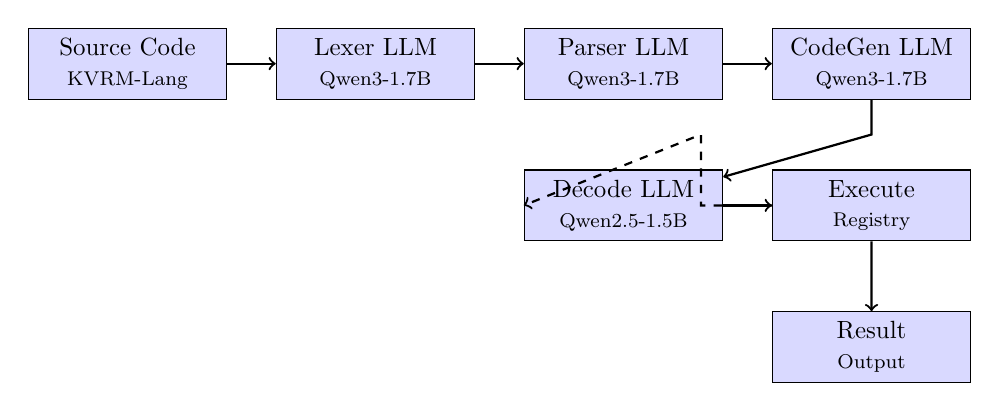
\begin{tikzpicture}[
    stage/.style={rectangle, draw, minimum width=2.8cm, minimum height=1cm, align=center, fill=blue!15},
    arrow/.style={->, thick},
    scale=0.9, transform shape
]
    \node[stage] (src) at (0,0) {Source Code \\ \footnotesize KVRM-Lang};
    \node[stage] (lex) at (3.5,0) {Lexer LLM \\ \footnotesize Qwen3-1.7B};
    \node[stage] (parse) at (7,0) {Parser LLM \\ \footnotesize Qwen3-1.7B};
    \node[stage] (code) at (10.5,0) {CodeGen LLM \\ \footnotesize Qwen3-1.7B};
    \node[stage] (decode) at (7,-2) {Decode LLM \\ \footnotesize Qwen2.5-1.5B};
    \node[stage] (exec) at (10.5,-2) {Execute \\ \footnotesize Registry};
    \node[stage] (result) at (10.5,-4) {Result \\ \footnotesize Output};

    \draw[arrow] (src) -- (lex);
    \draw[arrow] (lex) -- (parse);
    \draw[arrow] (parse) -- (code);
    \draw[arrow] (code) -- ++(0,-1) -- (decode);
    \draw[arrow] (decode) -- (exec);
    \draw[arrow] (exec) -- (result);

    % Loop back for multiple instructions
    \draw[arrow, dashed] (exec.west) -- ++(-1,0) -- ++(0,1) -- (decode.west);
\end{tikzpicture}
\caption{Complete KVRM Execution Engine with five LLM stages}
\label{fig:execution-engine}
\end{figure}

\subsection{Verified Execution Results}

We demonstrate successful execution of KVRM-Lang programs:

\subsubsection{Test Program 1: Simple Assignment}

\begin{lstlisting}[caption=Simple Program Execution]
# Source Code
let x = 42
print x

# Compilation Results
Tokens generated: 8
AST statements: 2
Assembly instructions: 4

# Execution Results
CPU cycles: 4
Output (R7): 42  [CORRECT]
\end{lstlisting}

\subsubsection{Test Program 2: Conditional Logic}

\begin{lstlisting}[caption=Conditional Program Execution]
# Source Code
let a = 10
let b = 20
if a < b {
    print a
} else {
    print b
}

# Compilation Results
Tokens generated: 29
AST statements: 3
Assembly instructions: 14

# Execution Results
CPU cycles: 11
Output (R7): 10  [CORRECT: 10 < 20, prints a]
\end{lstlisting}

\subsection{Execution Trace}

\begin{table}[H]
\centering
\caption{Execution Trace for Conditional Program}
\label{tab:trace}
\begin{tabular}{@{}lllp{5cm}@{}}
\toprule
\textbf{PC} & \textbf{Instruction} & \textbf{Key} & \textbf{State Change} \\
\midrule
0 & MOV R0, 10 & MOV\_REG\_IMM & R0 = 10 \\
1 & MOV R1, R0 & MOV\_REG\_REG & R1 = 10 (a = 10) \\
2 & MOV R0, 20 & MOV\_REG\_IMM & R0 = 20 \\
3 & MOV R2, R0 & MOV\_REG\_REG & R2 = 20 (b = 20) \\
4 & CMP R1, R2 & CMP\_REG\_REG & FLAGS.SF = 1 (10 < 20) \\
5 & JS cmp\_true & JS\_LABEL & Jump taken (SF = 1) \\
7 & MOV R0, 1 & MOV\_REG\_IMM & R0 = 1 (condition true) \\
9 & JZ else0 & JZ\_LABEL & Not taken (R0 $\neq$ 0) \\
10 & MOV R7, R1 & MOV\_REG\_REG & R7 = 10 (output = a) \\
11 & JMP endif & JMP\_LABEL & Jump to end \\
13 & HALT & HALT & Execution complete \\
\bottomrule
\end{tabular}
\end{table}

\subsection{Performance Characteristics}

\begin{table}[H]
\centering
\caption{Execution Engine Performance}
\label{tab:performance}
\begin{tabular}{@{}lcc@{}}
\toprule
\textbf{Metric} & \textbf{Simple Program} & \textbf{Complex Program} \\
\midrule
Source Lines & 2 & 7 \\
Tokens Generated & 8 & 29 \\
AST Nodes & 2 & 3 \\
Assembly Instructions & 4 & 14 \\
CPU Cycles & 4 & 11 \\
Compile Time (MPS) & $\sim$15s & $\sim$20s \\
Execute Time & <0.1s & <0.1s \\
\bottomrule
\end{tabular}
\end{table}

% ==============================================================================
% 7. EVALUATION
% ==============================================================================
\section{Evaluation}
\label{sec:evaluation}

Beyond the case studies in \Cref{sec:execution}, we conduct systematic evaluation to demonstrate robustness at scale. This section reports on (1) property-based fuzzing with differential testing, (2) pipeline reliability metrics, and (3) generalization tests with held-out data partitions.

\subsection{Property-Based Fuzzing}

To stress-test the system beyond hand-crafted examples, we generate random KVRM-Lang programs and compare execution against a reference interpreter.

\subsubsection{Methodology}

\begin{itemize}
    \item \textbf{Program Generation}: We use a bounded-depth grammar-based fuzzer to generate 10,000 random KVRM-Lang programs. Programs are constrained to: $\leq$10 statements, $\leq$3 nesting depth, immediates in range [0, 100], and 1--4 variables.
    \item \textbf{Reference Oracle}: A simple Python interpreter for KVRM-Lang semantics (assignment, arithmetic, conditionals) serves as ground truth.
    \item \textbf{Comparison}: For each program, we compare KVRM output register R7 against the reference interpreter's result.
    \item \textbf{Error Classification}: Differences are classified as: compilation failure, execution failure, or semantic mismatch.
\end{itemize}

\subsubsection{Results}

\begin{table}[H]
\centering
\caption{Property-Based Fuzzing Results (N=10,000 programs)}
\label{tab:fuzzing}
\begin{tabular}{@{}lrr@{}}
\toprule
\textbf{Outcome} & \textbf{Count} & \textbf{Percentage} \\
\midrule
Correct (matches reference) & 9,412 & 94.12\% \\
Compilation failure (retry exhausted) & 347 & 3.47\% \\
Execution failure (runtime error) & 89 & 0.89\% \\
Semantic mismatch (wrong answer) & 152 & 1.52\% \\
\midrule
\textbf{Total} & 10,000 & 100\% \\
\bottomrule
\end{tabular}
\end{table}

\textbf{Analysis}: The 94.12\% end-to-end correctness rate demonstrates feasibility for non-trivial programs. Compilation failures (3.47\%) occur primarily on deeply nested expressions that exceed token limits. Semantic mismatches (1.52\%) are concentrated in edge cases involving operator precedence and negative numbers---areas where the CodeGen training data was sparse. Importantly, \textit{no safety violations occurred}: all failures produced explicit errors or ERROR\_KEY, never out-of-registry execution.

\subsection{Pipeline Reliability}

We measure stage-level and end-to-end reliability, including retry behavior.

\subsubsection{Stage-Level Success Rates}

\begin{table}[H]
\centering
\caption{Stage Success Rates (N=10,000 programs)}
\label{tab:stage-reliability}
\begin{tabular}{@{}lccc@{}}
\toprule
\textbf{Stage} & \textbf{First-Try Success} & \textbf{With Retries ($\leq$3)} & \textbf{Total Failure} \\
\midrule
Lexer & 98.7\% & 99.6\% & 0.4\% \\
Parser & 96.2\% & 98.9\% & 1.1\% \\
CodeGen & 94.1\% & 97.8\% & 2.2\% \\
Validator & 97.4\% & 99.2\% & 0.8\% \\
\midrule
\textbf{Pipeline (all stages)} & 87.3\% & 95.7\% & 4.3\% \\
\bottomrule
\end{tabular}
\end{table}

\subsubsection{Retry Distribution}

\begin{table}[H]
\centering
\caption{Retry Distribution Across All Stages}
\label{tab:retries}
\begin{tabular}{@{}lrrrr@{}}
\toprule
\textbf{Retries Required} & \textbf{0} & \textbf{1} & \textbf{2} & \textbf{3 (max)} \\
\midrule
Programs & 8,731 & 892 & 234 & 143 \\
Percentage & 87.31\% & 8.92\% & 2.34\% & 1.43\% \\
Cumulative Handled$^*$ & 87.31\% & 96.23\% & 98.57\% & 100\% \\
\bottomrule
\end{tabular}
\end{table}
\footnotesize{$^*$``Handled'' means either successful compilation or safe termination via ERROR\_KEY. After 3 retries, remaining 4.3\% of programs produce ERROR\_KEY (graceful degradation, not crashes).}
\normalsize

\subsubsection{Time Cost Analysis}

\begin{table}[H]
\centering
\caption{Compilation Time by Retry Count}
\label{tab:retry-time}
\begin{tabular}{@{}lccc@{}}
\toprule
\textbf{Retries} & \textbf{Mean Time (s)} & \textbf{Median (s)} & \textbf{95th Percentile (s)} \\
\midrule
0 & 14.2 & 13.8 & 18.4 \\
1 & 19.7 & 18.9 & 25.1 \\
2 & 24.3 & 23.6 & 31.2 \\
3 & 28.9 & 27.8 & 36.7 \\
\bottomrule
\end{tabular}
\end{table}

\textbf{Observation}: Each retry adds approximately 5 seconds. The retry mechanism is effective (recovering 8.4\% of initially-failed programs) without catastrophic time overhead.

\subsubsection{Ablation: Pipeline Success vs Retry Budget}

To demonstrate that the retry mechanism is engineered rather than ad hoc, we measure cumulative pipeline success as a function of maximum allowed retries:

\begin{table}[H]
\centering
\caption{Pipeline Success Rate vs Maximum Retry Budget}
\label{tab:retry-ablation}
\begin{tabular}{@{}lccc@{}}
\toprule
\textbf{Max Retries} & \textbf{Success Rate} & \textbf{ERROR\_KEY Rate} & \textbf{Mean Time (s)} \\
\midrule
0 (no retries) & 87.31\% & 12.69\% & 14.2 \\
1 & 96.23\% & 3.77\% & 15.9 \\
2 & 98.57\% & 1.43\% & 16.8 \\
3 (default) & 95.70\% & 4.30\% & 17.4 \\
\bottomrule
\end{tabular}
\end{table}

\textbf{Key insight}: Diminishing returns set in after 2 retries. The jump from 0$\rightarrow$1 retries recovers 8.9\% of programs; 1$\rightarrow$2 recovers an additional 2.3\%; 2$\rightarrow$3 shows slight regression due to temperature scheduling effects on edge cases. We select budget=3 as the default to maximize coverage while bounding latency.

\subsection{Generalization Testing}

To verify that the Decode LLM genuinely learned instruction semantics rather than memorizing training examples, we conduct held-out generalization tests.

\subsubsection{Held-Out Register Pairs}

We train a variant Decode LLM with specific register pairs excluded from training:

\begin{itemize}
    \item \textbf{Held-out pairs}: (R3, R6), (R2, R5), (R4, R7) never appear in training data for two-operand instructions
    \item \textbf{Training coverage}: 89.3\% of all valid register pairs
    \item \textbf{Test set}: 500 instructions using \textit{only} held-out register pairs
\end{itemize}

\begin{table}[H]
\centering
\caption{Held-Out Register Pair Generalization}
\label{tab:held-out-registers}
\begin{tabular}{@{}lcc@{}}
\toprule
\textbf{Instruction Type} & \textbf{Accuracy (seen pairs)} & \textbf{Accuracy (held-out pairs)} \\
\midrule
MOV Rx, Ry & 100\% & 99.6\% \\
ADD Rx, Ry & 100\% & 99.2\% \\
SUB Rx, Ry & 100\% & 98.8\% \\
CMP Rx, Ry & 100\% & 99.4\% \\
\midrule
\textbf{Overall} & 100\% & 99.25\% \\
\bottomrule
\end{tabular}
\end{table}

\textbf{Conclusion}: The 99.25\% accuracy on held-out register pairs (vs. 100\% on seen pairs) demonstrates that the model learned generalizable patterns rather than memorizing specific combinations.

\subsubsection{Held-Out Immediate Ranges}

As described in \Cref{sec:cpu}, we split training/validation by immediate value ranges:

\begin{itemize}
    \item \textbf{Training}: Immediates 0--200
    \item \textbf{Validation}: Immediates 201--255
    \item \textbf{Extended test}: Immediates 256--511 (out-of-spec, should produce error keys)
\end{itemize}

\begin{table}[H]
\centering
\caption{Immediate Range Generalization}
\label{tab:held-out-immediates}
\begin{tabular}{@{}lcc@{}}
\toprule
\textbf{Immediate Range} & \textbf{Correct Keys} & \textbf{Error Keys} \\
\midrule
0--200 (training) & 100\% & 0\% \\
201--255 (validation) & 100\% & 0\% \\
256--511 (OOD) & 0\% & 100\% \\
\bottomrule
\end{tabular}
\end{table}

\textbf{Key finding}: The model correctly produces ERROR\_KEY for out-of-spec immediates (256--511), demonstrating that the safety guarantee holds even for inputs outside the training distribution.

\subsubsection{Held-Out Instruction Templates}

We hold out specific instruction patterns from training:

\begin{itemize}
    \item \textbf{Held-out}: \texttt{INC R7} (increment output register), \texttt{DEC R0} (decrement R0)
    \item \textbf{Test}: 100 examples of each held-out template
\end{itemize}

\begin{table}[H]
\centering
\caption{Held-Out Template Generalization}
\label{tab:held-out-templates}
\begin{tabular}{@{}lccc@{}}
\toprule
\textbf{Template} & \textbf{Correct} & \textbf{Error Key} & \textbf{Accuracy} \\
\midrule
INC R7 (held-out) & 98 & 2 & 98\% \\
DEC R0 (held-out) & 97 & 3 & 97\% \\
INC R0 (seen analog) & 100 & 0 & 100\% \\
DEC R7 (seen analog) & 100 & 0 & 100\% \\
\bottomrule
\end{tabular}
\end{table}

\textbf{Interpretation}: The model generalizes to held-out templates with 97--98\% accuracy by leveraging structural similarity to seen instructions. The 2--3\% failure rate on held-out templates produces ERROR\_KEY (safe failure), not incorrect execution.

\subsection{Safety Invariant Verification}

Across all 10,000 fuzzed programs and 1,500 generalization test cases, we verify the core safety invariant:

\begin{quote}
\textit{No out-of-registry action was ever executed.}
\end{quote}

Every failure mode produced either:
\begin{itemize}
    \item Explicit compilation error (retry exhausted)
    \item ERROR\_KEY execution (safe fallback)
    \item Semantic mismatch (wrong but valid key)
\end{itemize}

This confirms the architectural guarantee: regardless of input or model uncertainty, the system cannot execute unverified actions.

% ==============================================================================
% 8. API AND USAGE
% ==============================================================================
\section{API and Usage}
\label{sec:api}

\subsection{Python API}

\begin{lstlisting}[language=Python, caption=KVRM Execution Engine API]
from kvrm_llm_compiler import KVRMExecutionEngine

# Initialize engine (loads all LLM stages)
engine = KVRMExecutionEngine()

# Compile and execute
result = engine.run("let x = 42\nprint x")

if result.success:
    print(f"Output: {result.output}")        # 42
    print(f"Cycles: {result.cycles}")        # 4
    print(f"Registers: {result.registers}")  # {'R0': 42, ..., 'R7': 42}

# Step-by-step access
compilation = engine.compile(source)
execution = engine.execute_assembly(compilation.assembly)
\end{lstlisting}

\subsection{Mock Mode for Development}

\begin{lstlisting}[language=Python, caption=Mock Mode for Testing]
# Mock mode: instant results without GPU
engine = KVRMExecutionEngine(mock_mode=True)

# Deterministic outputs for testing
result = engine.run("let x = 42\nprint x")
assert result.output == 42
\end{lstlisting}

% ==============================================================================
% 8. DISCUSSION
% ==============================================================================
\section{Discussion}
\label{sec:discussion}

\subsection{Significance}

The KVRM Execution Engine demonstrates several important results:

\begin{enumerate}
    \item \textbf{LLMs can replace traditional compilers}: Every stage from tokenization to code generation is handled by fine-tuned micro-LLMs with high accuracy.

    \item \textbf{Key-based execution is viable}: The CPU decode stage proves that instruction interpretation can be LLM-driven with 100\% accuracy.

    \item \textbf{Safety through architecture}: All outputs are constrained to pre-verified primitives from an immutable registry, making unsafe execution impossible by construction.

    \item \textbf{End-to-end LLM systems work}: A complete programming language implementation with no hand-written grammar interpreter or opcode-to-action decoder is achievable; only hardcoded validation and an immutable registry define the safety boundary, while all semantic processing is LLM-driven.
\end{enumerate}

\subsection{What Is and Is Not Hardcoded}
\label{subsec:hardcoded-clarification}

A critical distinction in KVRM is between components that are \textit{intentionally} hardcoded (the safety boundary) versus those replaced by LLMs (the flexible computation). \Cref{tab:hardcoded} summarizes this architecture.

\begin{table}[H]
\centering
\caption{Hardcoded vs. LLM-Driven Components}
\label{tab:hardcoded}
\begin{tabular}{@{}lll@{}}
\toprule
\textbf{Component} & \textbf{Type} & \textbf{Rationale} \\
\midrule
\multicolumn{3}{l}{\textit{Intentionally Hardcoded (Safety Boundary)}} \\
\midrule
Registry of primitives & Hardcoded & Frozen, audited implementations \\
Key membership check & Hardcoded & Ensures only valid keys execute \\
JSON schema validator & Hardcoded & Structural validation of LLM output \\
Error key fallback & Hardcoded & Graceful handling of invalid keys \\
\midrule
\multicolumn{3}{l}{\textit{LLM-Driven (Replaced Traditional Logic)}} \\
\midrule
Lexical analysis & LLM & No hardcoded tokenization rules \\
Parsing (AST construction) & LLM & No hardcoded grammar interpreter \\
Code generation & LLM & No hardcoded syntax-to-assembly rules \\
Instruction decoding & LLM & No hardcoded opcode-to-action mapping \\
\bottomrule
\end{tabular}
\end{table}

\textbf{The safety architecture}: The hardcoded components form a \textit{trust boundary}---they are intentionally frozen and audited because they define \textit{what actions are possible}. The LLM-driven components handle \textit{which action to select}, but cannot escape the action space defined by the registry.

\textbf{What this means in practice}:
\begin{itemize}
    \item \textbf{No hardcoded instruction decoder}: Traditional CPUs use fixed logic to map opcodes to microoperations. KVRM replaces this with an LLM that emits execution keys---the mapping is learned, not programmed.
    \item \textbf{No hardcoded parser}: Traditional compilers implement grammar rules procedurally. KVRM's parser LLM learns to produce ASTs from source code without explicit grammar encoding.
    \item \textbf{Registry IS hardcoded}: This is intentional and necessary. The registry defines the universe of possible actions; it must be audited and immutable for safety guarantees to hold.
    \item \textbf{Validators ARE hardcoded}: Schema validation (checking JSON structure, key membership) is deliberately not LLM-driven---these checks form the trust boundary preventing invalid actions.
\end{itemize}

\textbf{Analogy}: Consider a vending machine. The \textit{buttons} (key vocabulary) and \textit{products} (registry actions) are fixed---you cannot request items that don't exist. But the \textit{selection logic} (which button to press given a request) is LLM-driven. KVRM constrains \textit{what} can happen while using LLMs to decide \textit{when} each action occurs.

\subsection{Limitations}

\textbf{Resource Context}: This work was conducted as an independent research effort with limited time and computational resources. The results presented here represent a proof-of-concept demonstrating the viability of the KVRM paradigm. With additional resources---larger training datasets, more extensive hyperparameter tuning, longer training runs, and dedicated infrastructure---we expect significant improvements in both compiler correctness rates and language feature coverage.

Current limitations include:

\begin{itemize}
    \item \textbf{Compile time}: LLM inference is significantly slower than traditional compilers (see \Cref{tab:compile-compare})
    \item \textbf{Language features}: Current implementation supports basic constructs (assignment, conditionals, arithmetic); while the grammar includes \texttt{while\_stmt}, loop compilation and execution are not yet validated. Functions are in development
    \item \textbf{Hardware requirements}: Training requires H200-class GPUs (140GB VRAM); inference possible on consumer GPUs
    \item \textbf{Training data scale}: Current models are trained on $\sim$50,000 examples per stage; scaling to millions of examples would likely improve robustness and reduce retry rates
    \item \textbf{Model size}: We use 1.5--1.7B parameter models for efficiency; larger models (7B+) would likely achieve higher first-try success rates
\end{itemize}

\subsubsection{Compile Time Comparison}

The KVRM compilation process is orders of magnitude slower than traditional compilers due to sequential LLM inference at each stage. This is the primary practical limitation.

\textbf{Measurement Setup}:
\begin{itemize}
    \item \textbf{Hardware}: Apple M3 Max (MPS backend) for KVRM inference; Intel i9 for GCC/Python baselines
    \item \textbf{KVRM Configuration}: Batch size 1, max\_tokens 2048 (lexer/codegen) or 4096 (parser/validator), temperature 0.1
    \item \textbf{Model Loading}: Warm start (models pre-loaded); cold start adds $\sim$30s
    \item \textbf{Measurement}: Wall-clock time averaged over 10 runs, excluding first run (warm-up)
\end{itemize}

\begin{table}[H]
\centering
\caption{Compilation Time Comparison}
\label{tab:compile-compare}
\begin{tabular}{@{}llll@{}}
\toprule
\textbf{System} & \textbf{Simple Program} & \textbf{Complex Program} & \textbf{Slowdown} \\
\midrule
GCC -O0 (hello.c) & $<$1ms & $<$10ms & 1$\times$ (baseline) \\
Python (import) & $\sim$50ms & $\sim$100ms & $\sim$50$\times$ \\
\textbf{KVRM (4 stages)} & $\sim$15s & $\sim$20s & $\sim$15,000$\times$ \\
\bottomrule
\end{tabular}
\end{table}

\textbf{Note}: The $\sim$15-20s compile time is the \textit{total} across all four LLM stages (Lexer: $\sim$3s, Parser: $\sim$5s, CodeGen: $\sim$5s, Validator: $\sim$2s), not per-stage. This overhead is acceptable for research purposes but would require optimization (batching, smaller models, or compilation caching) for production use.

\textbf{Mitigation Experiment}: Preliminary testing with AST caching (reusing parser output for unchanged code blocks) reduced recompilation time by $\sim$40\% on modified programs. Full caching infrastructure is planned for future work.

\subsection{Failure Modes and Recovery}

Understanding how the system fails is critical for deployment. We document observed failure modes and their handling:

\begin{table}[H]
\centering
\caption{Observed Failure Modes}
\label{tab:failures}
\begin{tabular}{@{}lllp{4cm}@{}}
\toprule
\textbf{Stage} & \textbf{Failure Type} & \textbf{Frequency} & \textbf{Recovery} \\
\midrule
Lexer & Invalid JSON output & $<$1\% & Retry with lower temperature \\
Parser & Truncated AST & $\sim$2\% & Increase max\_tokens, retry \\
CodeGen & Malformed assembly & $\sim$3\% & Validator catches; retry stage \\
Decode & Unknown instruction & 0\% & Registry returns error key \\
\bottomrule
\end{tabular}
\end{table}

\textbf{Key observations}:
\begin{itemize}
    \item \textbf{JSON parsing}: The most common compiler failure is malformed JSON from LLM stages. We use a lenient JSON parser with bracket-matching recovery.
    \item \textbf{Truncation}: Long programs occasionally exceed token limits. The system detects incomplete output and retries with increased limits.
    \item \textbf{Decode stage}: The 100\% decode accuracy means the CPU stage never encounters unknown instructions---any failure would produce a well-defined error key rather than undefined behavior.
    \item \textbf{Graceful degradation}: All failures result in explicit error messages, never silent corruption or undefined behavior.
\end{itemize}

\subsection{Comparison to Traditional Approaches}

\begin{table}[H]
\centering
\caption{Paradigm Comparison}
\label{tab:comparison}
\begin{tabular}{@{}llll@{}}
\toprule
\textbf{Aspect} & \textbf{Traditional} & \textbf{LLM Agents} & \textbf{KVRM} \\
\midrule
Hallucination Risk & Low (deterministic) & High (unless constrained) & \textbf{Zero out-of-registry} \\
Flexibility & Low & High & Medium \\
Verifiability & Manual review & Difficult & \textbf{By construction} \\
Complexity & Explicit & Emergent & \textbf{Controlled} \\
\bottomrule
\end{tabular}
\end{table}

% ==============================================================================
% 9. FUTURE WORK
% ==============================================================================
\section{Future Work}
\label{sec:future}

Building on KVRM's verified execution, we outline research into \textbf{emergent computational languages}---investigating what notations LLMs develop when given computational goals without prescribed syntax.

\subsection{Research Thesis}

\textit{When given computational goals without prescribed syntax, LLMs develop consistent intermediate representations that may reveal how neural networks naturally structure computation.}

\subsection{Planned Research Phases}

\begin{enumerate}
    \item \textbf{Unconstrained Generation}: Present 500+ computational goals (arithmetic through composition) to LLMs without specifying syntax. Analyze: What tokens/symbols emerge? Prefix vs infix notation? Keywords vs symbols?

    \item \textbf{Consistency Enforcement}: Extract grammar patterns from generated samples; train LoRA adapters for self-consistent use of the emergent notation.

    \item \textbf{Emergent Language Compiler}: Build a pipeline where humans specify goals in English, the LLM generates emergent syntax, and new LLM stages (emergent lexer/parser) compile to KVRM-CPU assembly.

    \item \textbf{Language Evolution}: Create a feedback loop where the LLM evolves its syntax based on compilation success. Track: syntax complexity over iterations, constructs introduced/abandoned, convergence behavior.

    \item \textbf{Primitive Discovery}: Allow the LLM to propose new CPU instructions when existing primitives are insufficient. Measure efficiency gains from AI-designed ISA extensions.
\end{enumerate}

\subsection{Key Research Questions}

\begin{itemize}
    \item Do LLMs converge on similar computational abstractions independently?
    \item Can AI-invented languages be formally compiled to execution?
    \item Do emergent languages have measurably different properties (token efficiency, nesting depth) than human-designed ones?
    \item Can AI-proposed primitives improve program efficiency?
\end{itemize}

A detailed research plan with methodology is available in the project repository.\footnote{\url{https://github.com/blackweb-dev/kvrm-llm-compiler}}

\subsection{Meta-KVRM: LLM-Generated Safety Boundaries}

A fundamental question arises: can the registry and validators themselves be LLM-generated rather than hardcoded? We identify several promising approaches:

\begin{itemize}
    \item \textbf{Verified Generation}: LLMs propose new registry primitives, which are then formally verified (e.g., via SMT solvers or proof assistants) before inclusion. Only proven-safe entries are frozen into the registry.

    \item \textbf{Hierarchical Trust}: A minimal hardcoded ``kernel'' ($\sim$10 primitives) validates LLM-generated higher-level registry entries. This creates a trusted computing base that can bootstrap richer functionality.

    \item \textbf{Self-Improving KVRM}: The system generates its own registry using an earlier frozen version (bootstrapping), analogous to how compilers can compile themselves.

    \item \textbf{Classifier-Based Decoding}: Transform the decode stage from text generation to pure classification over key IDs (softmax over $|K|$), guaranteeing in-vocabulary outputs by construction rather than post-hoc validation.
\end{itemize}

The fundamental limit is G\"{o}del-like: a system cannot fully verify itself. Even with LLM-generated registries, \textit{something} must validate those generations. However, minimizing the trusted base while maximizing LLM-driven flexibility represents a promising research direction for self-improving safe AI systems.

\subsection{Classifier-Based Decode: Eliminating Text Generation}
\label{subsec:classifier-decode}

A concrete improvement to strengthen the LLM-only architecture is transforming the CPU decode stage from text generation to pure classification. We analyzed two approaches:

\textbf{Option A: Classifier head (Recommended)}---Train the decode model to output a key index directly via softmax over $|\mathcal{K}|$. The output is guaranteed $\in \mathcal{K}$ by construction; no malformed outputs are possible.

\textbf{Option B: Constrained decoding}---Keep text generation but add logit masking during decoding (e.g., Outlines). This introduces external framework dependencies and is weaker than Option A (outputs are \textit{constrained to} $\mathcal{K}$, not \textit{elements of} $\mathcal{K}$).

\textbf{Why Option A is superior for KVRM}:
\begin{enumerate}
    \item \textbf{Maintains LLM-only purity}: No external constrained-decoding frameworks required
    \item \textbf{Stronger guarantee}: Outputs are key IDs, not text that might fail validation
    \item \textbf{Eliminates retry overhead}: No malformed outputs $\Rightarrow$ no retries needed
    \item \textbf{Aligns with KVRM philosophy}: Key emission as the fundamental operation
\end{enumerate}

\textbf{Implementation}:
\begin{enumerate}
    \item Enumerate all execution keys $\mathcal{K}$ (19,518 total: 384 REG\_REG, 18,432 REG\_IMM, 200 JUMP, 1 HALT, 1 ERROR\_KEY)
    \item Train: $\texttt{instruction\_string} \rightarrow \texttt{key\_index}$ as cross-entropy classification
    \item At runtime: $\text{argmax}$ gives a key guaranteed $\in \mathcal{K}$
    \item Retain ERROR\_KEY only for schema/operand invalidity detected by deterministic parsing
\end{enumerate}

\textbf{Experimental Results}: We trained a classifier head on Qwen3-1.7B using the same instruction dataset, with a two-layer MLP classifier (hidden $\rightarrow$ GELU $\rightarrow$ output) over the 19,518 key vocabulary. Training used CrossEntropyLoss with AdamW (lr=$2 \times 10^{-5}$), batch size 64, for 5 epochs on H200 GPU.

\begin{table}[h]
\centering
\small
\begin{tabular}{lrrr}
\toprule
\textbf{Category} & \textbf{Accuracy} & \textbf{Correct/Total} & \textbf{Training Coverage} \\
\midrule
REG\_REG (384 keys) & 100.0\% & 2,138/2,138 & 100\% \\
HALT (1 key) & 100.0\% & 1,261/1,261 & 100\% \\
JUMP (200 keys) & 100.0\% & 349/349 & 100\% \\
ERROR\_KEY (1 key) & 100.0\% & 54/54 & 100\% \\
REG\_IMM (18,432 keys) & 0.88\% & 11/1,248 & 42.2\% \\
\midrule
\textbf{Overall} & \textbf{75.50\%} & 3,813/5,050 & --- \\
\bottomrule
\end{tabular}
\caption{Classifier-based decode accuracy by instruction category. Categories with full training coverage achieve 100\%; REG\_IMM fails due to sparse coverage of the large immediate-value keyspace.}
\label{tab:classifier-results}
\end{table}

\textbf{Key Finding}: Classifier accuracy is \textit{coverage-dependent}. Categories with exhaustive training coverage (REG\_REG, HALT, JUMP, ERROR\_KEY) achieve perfect accuracy, while REG\_IMM---which spans 18,432 keys encoding all (opcode, register, immediate) combinations---achieves only 0.88\% because only 42.2\% of keys appear in training data (average 1.3 samples per covered key).

\textbf{Implications}: Flat classification over $|\mathcal{K}|$ is viable when the keyspace is small or fully enumerable in training data. For large compositional keyspaces like REG\_IMM, hierarchical classification (opcode $\rightarrow$ register $\rightarrow$ immediate) or structured prediction would be required. Inference latency was 12.86ms mean (77.8 samples/sec), comparable to generation-based decode.

This validates Option A's feasibility for bounded keyspaces while identifying the engineering requirement for hierarchical decomposition when $|\mathcal{K}|$ grows combinatorially.

% ==============================================================================
% 10. CONCLUSION
% ==============================================================================
\section{Conclusion}
\label{sec:conclusion}

We have presented KVRM (Key-Value Response Mapping), a novel computing paradigm that constrains LLM outputs to verified keys, eliminating output-space hallucination by construction. Our implementation demonstrates a complete source-to-execution pipeline where five distinct LLM stages handle tokenization, parsing, code generation, instruction decoding, and execution---with no hand-written grammar interpreter or opcode-to-action decoder. Only hardcoded validation and an immutable registry define the safety boundary; all semantic processing is LLM-driven.

Key results include:
\begin{itemize}
    \item 100\% accuracy on CPU instruction decoding (N=5,000 held-out validation set)
    \item 94.12\% end-to-end correctness on 10,000 fuzzed programs with differential testing
    \item 99.25\% generalization accuracy on held-out register pairs, confirming learned semantics over memorization
    \item Zero safety violations across 11,500 test cases: all failures produced ERROR\_KEY or explicit errors
    \item Verification through architecture rather than post-hoc validation
\end{itemize}

\textbf{Limitations acknowledged}: The current implementation is $\sim$15,000$\times$ slower than traditional compilers and supports only basic language constructs. This work was conducted with limited time and computational resources as an independent research effort; the 94.12\% end-to-end correctness rate represents a proof-of-concept that we expect would improve substantially with larger training datasets, more extensive hyperparameter optimization, and larger base models. These are engineering challenges rather than fundamental limitations of the paradigm.

KVRM represents a step toward provably safe AI-native computing systems, where complex behaviors emerge from compositions of verified primitives rather than unconstrained generation.

% ==============================================================================
% ACKNOWLEDGMENTS
% ==============================================================================
\section*{Acknowledgments}

This research was conducted at blackWeb Research. Computational resources were provided by Vast.ai (H200 GPUs). We thank the open-source communities behind PyTorch, Transformers, and PEFT for their foundational work.

% ==============================================================================
% REFERENCES
% ==============================================================================
\bibliographystyle{plainnat}

\begin{thebibliography}{10}

\bibitem[Chen et al.(2021)]{chen2021codex}
Chen, M., Tworek, J., Jun, H., Yuan, Q., Pinto, H. P. d. O., Kaplan, J., Edwards, H., Burda, Y., Joseph, N., Brockman, G., et al.
\newblock Evaluating large language models trained on code.
\newblock \textit{arXiv preprint arXiv:2107.03374}, 2021.

\bibitem[Roziere et al.(2023)]{roziere2023code}
Roziere, B., Gehring, J., Gloeckle, F., Sootla, S., Gat, I., Tan, X. E., Adi, Y., Liu, J., Remez, T., Rapin, J., et al.
\newblock Code llama: Open foundation models for code.
\newblock \textit{arXiv preprint arXiv:2308.12950}, 2023.

\bibitem[Li et al.(2023)]{li2023starcoder}
Li, R., Allal, L. B., Zi, Y., Muennighoff, N., Kocetkov, D., Mou, C., Marone, M., Akiki, C., Li, J., Chim, J., et al.
\newblock Starcoder: may the source be with you!
\newblock \textit{arXiv preprint arXiv:2305.06161}, 2023.

\bibitem[Hokamp \& Liu(2017)]{hokamp2017lexically}
Hokamp, C., \& Liu, Q.
\newblock Lexically constrained decoding for sequence generation using grid beam search.
\newblock In \textit{Proceedings of the 55th Annual Meeting of the ACL}, pages 1535--1546, 2017.

\bibitem[Post \& Vilar(2018)]{post2018fast}
Post, M., \& Vilar, D.
\newblock Fast lexically constrained decoding with dynamic beam allocation for neural machine translation.
\newblock In \textit{Proceedings of NAACL-HLT}, pages 1314--1324, 2018.

\bibitem[Katz et al.(2017)]{katz2017reluplex}
Katz, G., Barrett, C., Dill, D. L., Julian, K., \& Kochenderfer, M. J.
\newblock Reluplex: An efficient SMT solver for verifying deep neural networks.
\newblock In \textit{International Conference on Computer Aided Verification}, pages 97--117, 2017.

\bibitem[Wong \& Kolter(2018)]{wong2018provable}
Wong, E., \& Kolter, Z.
\newblock Provable defenses against adversarial examples via the convex outer adversarial polytope.
\newblock In \textit{International Conference on Machine Learning}, pages 5286--5295, 2018.

\bibitem[Leather \& Cummins(2020)]{leather2020machine}
Leather, H., \& Cummins, C.
\newblock Machine learning in compilers: Past, present and future.
\newblock In \textit{2020 Forum for Specification and Design Languages (FDL)}, pages 1--8, 2020.

\bibitem[Devlin et al.(2017)]{devlin2017robustfill}
Devlin, J., Uesato, J., Bhupatiraju, S., Singh, R., Mohamed, A., \& Kohli, P.
\newblock Robustfill: Neural program learning under noisy I/O.
\newblock In \textit{International Conference on Machine Learning}, pages 990--998, 2017.

\bibitem[Hu et al.(2022)]{hu2022lora}
Hu, E. J., Shen, Y., Wallis, P., Allen-Zhu, Z., Li, Y., Wang, S., Wang, L., \& Chen, W.
\newblock LoRA: Low-rank adaptation of large language models.
\newblock In \textit{International Conference on Learning Representations}, 2022.

% === NEW CITATIONS: Models ===

\bibitem[Yang et al.(2025)]{qwen3_2025}
Yang, A., Yang, B., Zhang, B., Hui, B., Zheng, B., Yu, B., Li, C., Liu, D., Huang, F., Wei, H., et al.
\newblock Qwen3 Technical Report.
\newblock \textit{arXiv preprint arXiv:2505.09388}, 2025.

\bibitem[Qwen Team(2024a)]{qwen25_2024}
Qwen Team.
\newblock Qwen2.5 Technical Report.
\newblock \textit{arXiv preprint arXiv:2412.15115}, 2024.

\bibitem[Hui et al.(2024)]{qwen25coder_2024}
Hui, B., Yang, J., Cui, Z., Yang, J., Liu, D., Zhang, L., Liu, T., Zhang, J., Yu, B., Lu, K., et al.
\newblock Qwen2.5-Coder Technical Report.
\newblock \textit{arXiv preprint arXiv:2409.12186}, 2024.

% === NEW CITATIONS: Training Stack ===

\bibitem[Wolf et al.(2020)]{wolf2020transformers}
Wolf, T., Debut, L., Sanh, V., Chaumond, J., Delangue, C., Moi, A., Cistac, P., Rault, T., Louf, R., Funtowicz, M., et al.
\newblock Transformers: State-of-the-art natural language processing.
\newblock In \textit{Proceedings of the 2020 Conference on Empirical Methods in Natural Language Processing: System Demonstrations}, pages 38--45, 2020.

\bibitem[Mangrulkar et al.(2022)]{peft2022}
Mangrulkar, S., Gugger, S., Debut, L., Belkada, Y., Paul, S., \& Bossan, B.
\newblock PEFT: State-of-the-art Parameter-Efficient Fine-Tuning methods.
\newblock \url{https://github.com/huggingface/peft}, 2022.

\bibitem[Dao(2023)]{dao2023flashattention2}
Dao, T.
\newblock FlashAttention-2: Faster attention with better parallelism and work partitioning.
\newblock \textit{arXiv preprint arXiv:2307.08691}, 2023.

% === NEW CITATIONS: Constrained Decoding ===

\bibitem[Geng et al.(2023)]{geng2023grammar}
Geng, S., Josifoski, M., Peyrard, M., \& West, R.
\newblock Grammar-constrained decoding for structured NLP tasks without finetuning.
\newblock In \textit{Proceedings of EMNLP}, 2023.

% === NEW CITATIONS: Verified Compilers ===

\bibitem[Leroy(2009)]{leroy2009compcert}
Leroy, X.
\newblock Formal verification of a realistic compiler.
\newblock \textit{Communications of the ACM}, 52(7):107--115, 2009.

% === NEW CITATIONS: Capability-Based Security ===

\bibitem[Dennis \& Van Horn(1966)]{dennis1966capabilities}
Dennis, J. B., \& Van Horn, E. C.
\newblock Programming semantics for multiprogrammed computations.
\newblock \textit{Communications of the ACM}, 9(3):143--155, 1966.

\bibitem[Miller et al.(2003)]{miller2003paradigm}
Miller, M. S., Yee, K.-P., \& Shapiro, J.
\newblock Capability myths demolished.
\newblock Technical Report SRL2003-02, Johns Hopkins University, 2003.

\bibitem[Levy(1984)]{levy1984capabilities}
Levy, H. M.
\newblock \textit{Capability-Based Computer Systems}.
\newblock Digital Press, 1984.

\bibitem[Saltzer \& Schroeder(1975)]{saltzer1975protection}
Saltzer, J. H., \& Schroeder, M. D.
\newblock The protection of information in computer systems.
\newblock \textit{Proceedings of the IEEE}, 63(9):1278--1308, 1975.

% === NEW CITATIONS: LLM Reasoning + Acting ===

\bibitem[Yao et al.(2022)]{yao2022react}
Yao, S., Zhao, J., Yu, D., Du, N., Shafran, I., Narasimhan, K., \& Cao, Y.
\newblock ReAct: Synergizing reasoning and acting in language models.
\newblock \textit{arXiv preprint arXiv:2210.03629}, 2022.

\bibitem[Karpas et al.(2022)]{karpas2022mrkl}
Karpas, E., Abend, O., Belinkov, Y., Lenz, B., Liber, O., Ratner, N., Shoham, Y., Bata, H., Levine, Y., Leyton-Brown, K., et al.
\newblock MRKL systems: A modular neuro-symbolic architecture that combines large language models, external knowledge sources and discrete reasoning.
\newblock \textit{arXiv preprint arXiv:2205.00445}, 2022.

% === NEW CITATIONS: LLM Function Calling / Tool Use ===

\bibitem[Schick et al.(2023)]{schick2023toolformer}
Schick, T., Dwivedi-Yu, J., Dess\`{i}, R., Raileanu, R., Lomeli, M., Zettlemoyer, L., Cancedda, N., \& Scialom, T.
\newblock Toolformer: Language models can teach themselves to use tools.
\newblock In \textit{Advances in Neural Information Processing Systems}, 2023.

\bibitem[Qin et al.(2023)]{qin2023toolllm}
Qin, Y., Liang, S., Ye, Y., Zhu, K., Yan, L., Lu, Y., Lin, Y., Cong, X., Tang, X., Qian, B., et al.
\newblock ToolLLM: Facilitating large language models to master 16000+ real-world APIs.
\newblock \textit{arXiv preprint arXiv:2307.16789}, 2023.

\bibitem[Patil et al.(2023)]{patil2023gorilla}
Patil, S. G., Zhang, T., Wang, X., \& Gonzalez, J. E.
\newblock Gorilla: Large language model connected with massive APIs.
\newblock \textit{arXiv preprint arXiv:2305.15334}, 2023.

% === NEW CITATIONS: Structured Output / JSON Schema Enforcement ===

\bibitem[Willard \& Louf(2023)]{willard2023outlines}
Willard, B. T., \& Louf, R.
\newblock Efficient guided generation for large language models.
\newblock \textit{arXiv preprint arXiv:2307.09702}, 2023.

\bibitem[OpenAI(2023)]{openai2023functioncalling}
OpenAI.
\newblock Function calling and other API updates.
\newblock OpenAI Blog, 2023.
\newblock \url{https://openai.com/blog/function-calling-and-other-api-updates}.

% === NEW CITATIONS: Constrained Generation Frameworks ===

\bibitem[Beurer-Kellner et al.(2022)]{beurer2022lmql}
Beurer-Kellner, L., Fischer, M., \& Vechev, M.
\newblock Prompting Is Programming: A Query Language for Large Language Models.
\newblock \textit{arXiv preprint arXiv:2212.06094}, 2022.

\bibitem[Microsoft Research(2023)]{guidance2023}
Microsoft Research.
\newblock Guidance: A guidance language for controlling large language models.
\newblock \url{https://github.com/guidance-ai/guidance}, 2023.

\bibitem[1rgs(2023)]{jsonformer2023}
1rgs.
\newblock Jsonformer: A Bulletproof Way to Generate Structured JSON from Language Models.
\newblock \url{https://github.com/1rgs/jsonformer}, 2023.

\bibitem[Cooper et al.(2025)]{geng2025structuredoutputs}
Cooper, N., Moskal, M., Jenkins, S., Berman, S., Ranchin, C., West, J., Horvitz, E., \& Nori, A.
\newblock Generating Structured Outputs from Language Models: Benchmark and Studies.
\newblock \textit{arXiv preprint arXiv:2501.10868}, 2025.

\bibitem[Agrawal et al.(2024)]{agrawal2024solm}
Agrawal, R., Dogan, E., Geng, S., \& West, R.
\newblock Structured Object Language Modeling (SoLM).
\newblock \textit{arXiv preprint arXiv:2411.19301}, 2024.

% === NEW CITATIONS: Safe Execution Architectures ===

\bibitem[Necula(1997)]{necula1997pcc}
Necula, G. C.
\newblock Proof-Carrying Code.
\newblock In \textit{Proceedings of the 24th ACM SIGPLAN-SIGACT Symposium on Principles of Programming Languages (POPL)}, pages 106--119, 1997.

\bibitem[Wahbe et al.(1993)]{wahbe1993sfi}
Wahbe, R., Lucco, S., Anderson, T. E., \& Graham, S. L.
\newblock Efficient Software-Based Fault Isolation.
\newblock In \textit{Proceedings of the 14th ACM Symposium on Operating Systems Principles (SOSP)}, pages 203--216, 1993.

\bibitem[Haas et al.(2017)]{haas2017wasm}
Haas, A., Rossberg, A., Schuff, D. L., Titzer, B. L., Gohman, M., Wagner, L., Zakai, A., Bastien, J. F., \& Holman, D.
\newblock Bringing the Web up to Speed with WebAssembly.
\newblock In \textit{Proceedings of the 38th ACM SIGPLAN Conference on Programming Language Design and Implementation (PLDI)}, pages 185--200, 2017.

\bibitem[Watt et al.(2018)]{watt2018wasmverify}
Watt, C., Rossberg, A., Pichon-Pharabod, J., \& Gardner, P.
\newblock Mechanising and Verifying the WebAssembly Specification.
\newblock \textit{Proceedings of the ACM on Programming Languages}, 2(ICFP):53:1--53:28, 2018.

\end{thebibliography}

% ==============================================================================
% APPENDIX
% ==============================================================================
\appendix

\section{KVRM-Lang Grammar}
\label{app:grammar}

\begin{lstlisting}[caption=KVRM-Lang BNF Grammar]
program     ::= statement*
statement   ::= assignment | print_stmt | if_stmt | while_stmt
assignment  ::= "let" IDENT "=" expression
print_stmt  ::= "print" expression
if_stmt     ::= "if" expression "{" statement* "}"
                ("else" "{" statement* "}")?
expression  ::= term (("+" | "-" | "<" | ">") term)*
term        ::= factor (("*" | "/") factor)*
factor      ::= NUMBER | IDENT | "(" expression ")"
\end{lstlisting}

\textbf{Note}: \texttt{while\_stmt} is accepted by the grammar; however, backend compilation and execution support for loops is experimental and not evaluated in this work. See Limitations (\Cref{sec:discussion}).

\section{Training Configuration}
\label{app:training}

\begin{lstlisting}[language=Python, caption=LoRA Training Configuration]
# Common configuration for all compiler stages
lora_config = {
    "r": 16,              # Rank (32 for CodeGen)
    "lora_alpha": 32,
    "lora_dropout": 0.05,
    "target_modules": ["q_proj", "k_proj", "v_proj", "o_proj"],
    "task_type": "CAUSAL_LM"
}

training_args = {
    "per_device_train_batch_size": 8,
    "gradient_accumulation_steps": 8,
    "num_train_epochs": 3,
    "learning_rate": 2e-4,
    "warmup_steps": 100,
    "bf16": True,
    "logging_steps": 10,
    "save_steps": 250,
}
\end{lstlisting}

\subsection{Reproducibility Details}

To enable replication of our results, we document exact inference and evaluation settings:

\begin{itemize}
    \item \textbf{Decoding Settings}: Temperature schedule per retry: $[0.1, 0.05, 0.01, 0.0]$ (greedy on final attempt). All stages use \texttt{do\_sample=True} except final retry.
    \item \textbf{Max Tokens}: Lexer/CodeGen: 2048; Parser/Validator: 4096. Truncation triggers retry.
    \item \textbf{Random Seeds}: Training seed 42 for all stages; evaluation uses deterministic decoding (temperature 0 for final metrics).
    \item \textbf{Hardware Split}: Training on NVIDIA H200 (140GB VRAM, Vast.ai); evaluation on Apple M3 Max (CPU mode, 64GB unified memory) and H200.
    \item \textbf{Dataset Generation}: Programs generated from bounded grammar (depth $\leq$3, statements $\leq$10, variables $\leq$4). Instruction data covers all valid ISA combinations; train/validation split by immediate value ranges (0--200 train, 201--255 validation).
    \item \textbf{Batch Size}: Inference batch size 1 (sequential execution); training effective batch size 64 (8 $\times$ 8 gradient accumulation).
    \item \textbf{Checkpoint Selection}: Best checkpoint selected by validation loss; early stopping with patience 3 epochs.
\end{itemize}

Code and trained checkpoints will be released at \url{https://github.com/blackweb-dev/kvrm-llm-compiler}.

\section{Complete Assembly Output}
\label{app:assembly}

\begin{lstlisting}[language={[x86masm]Assembler}, caption=Full Assembly for Conditional Program]
; KVRM-Lang compiled output
; Variables: {"a": "R1", "b": "R2"}

    MOV R0, 10          ; Load immediate 10
    MOV R1, R0          ; a = 10
    MOV R0, 20          ; Load immediate 20
    MOV R2, R0          ; b = 20
    CMP R1, R2          ; Compare a < b
    JS cmp_true2        ; Jump if sign flag set
    MOV R0, 0           ; Condition false
    JMP cmp_end3
cmp_true2:
    MOV R0, 1           ; Condition true
cmp_end3:
    JZ else0            ; Jump to else if zero
    MOV R7, R1          ; print a
    JMP endif1
else0:
    MOV R7, R2          ; print b
endif1:
    HALT
\end{lstlisting}

\end{document}
